These methods lack intrinsic motivation in the zero reward environment (Except prior-BDQN) and introduce considerable computational overhead. 

In this work, we use the SGLD to draw samples from the posterior distribution during training the value function. There are a number of variants of SGLD, such as pre-condiction \cite{pSGLD}, SGHMC \cite{SGHMC}, SGFS\cite{SGFS}, etc. The pre-condiction SGLD can be seen as a variant of RMSprop and has as almost equal number of operations, and been used as the sampler in this work. Because SGLD can be seen as accumulatng Gaussian noise during the optimization process, our method has similarities with parameter noise. The difference is that we add accumulated noise to the critic by SGLD, while they only add one-time noise to the actor when rollout samples. On the other hand, in prior-BDQN, they prepare a set of "prior function" in advance then select some of them to add on Q-value function during training, while in our algorithm there only have a single-head network with accumulated noise so that our method is more computational efficient.

\begin{figure*}[htb]
   \centering
      \subfigure[$\alpha = 0$]{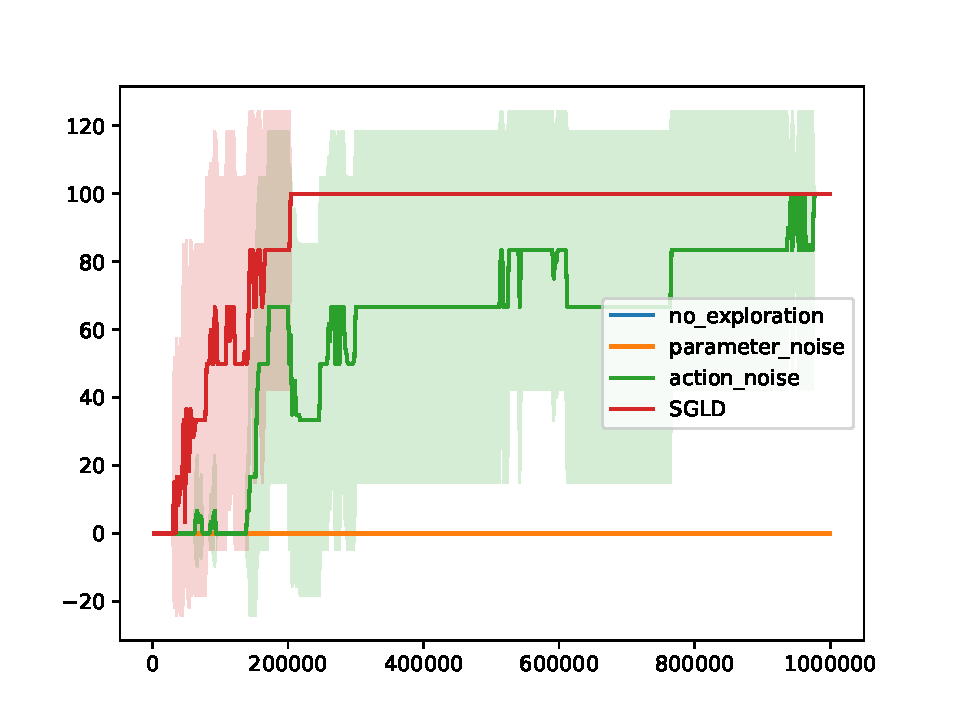
\includegraphics[width=85pt]{figs/MC0.pdf}}
      \subfigure[$\alpha = 0.1$]{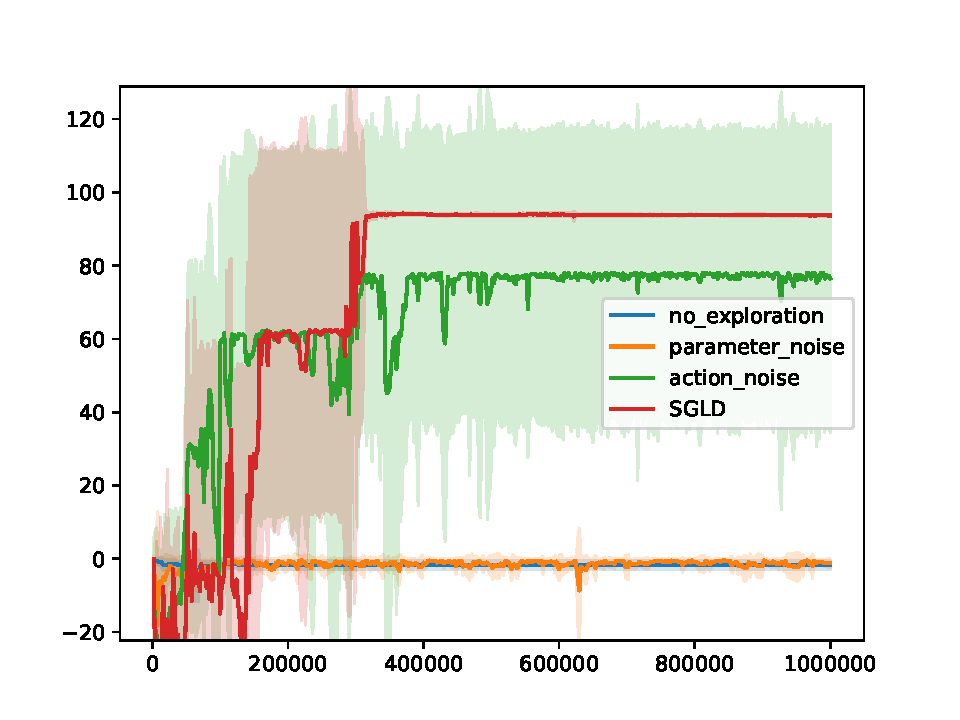
\includegraphics[width=85pt]{figs/MC.pdf}}
      \subfigure[$\alpha = 0.2$]{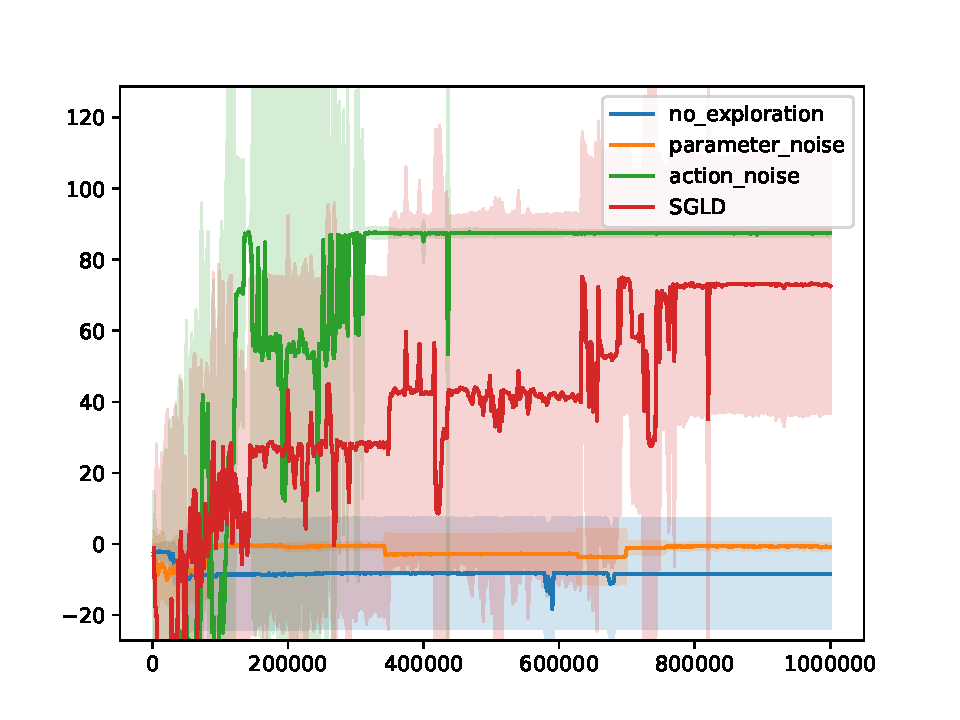
\includegraphics[width=85pt]{figs/MC0_2.pdf}}
      \subfigure[$\alpha = 0.5$]{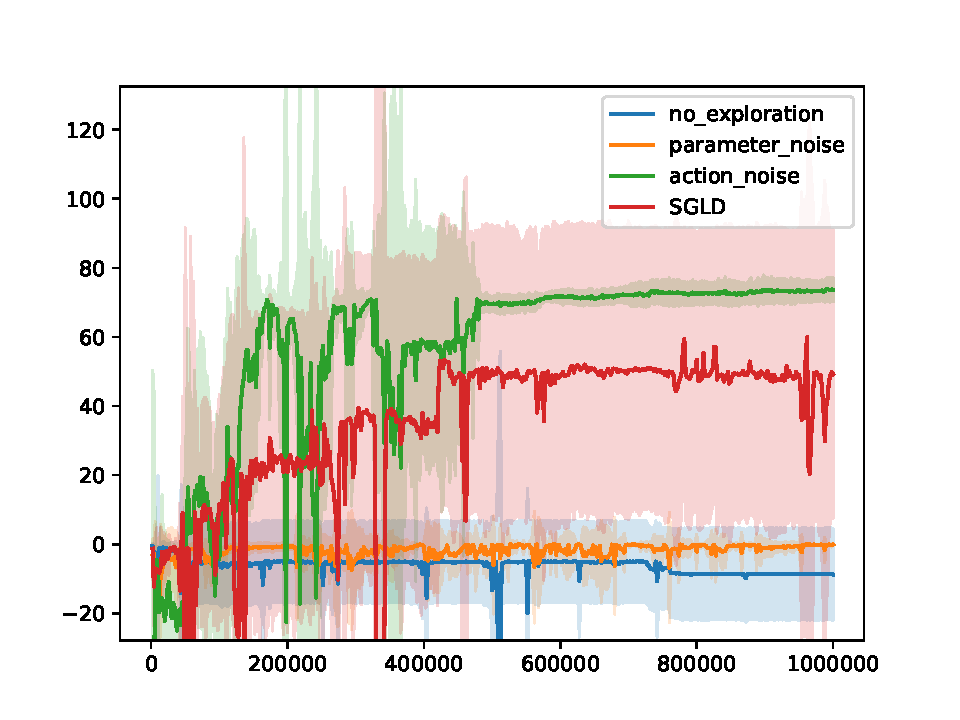
\includegraphics[width=85pt]{figs/MC0_5.pdf}}
      \subfigure[$\alpha = 1$]{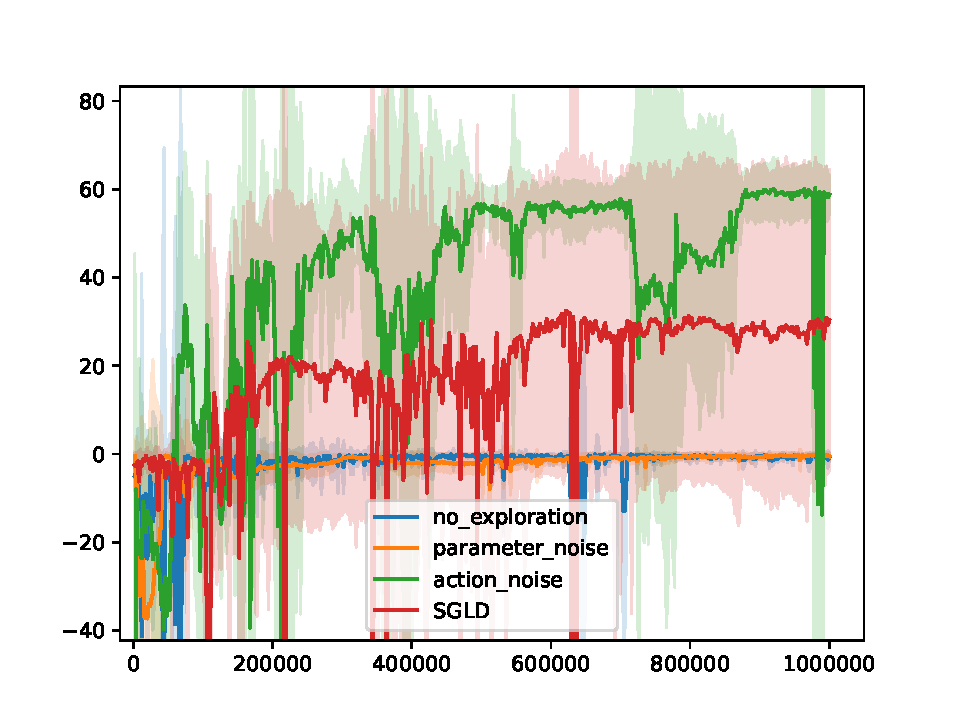
\includegraphics[width=85pt]{figs/MC1.pdf}}
      \subfigure[$\alpha = 0$]{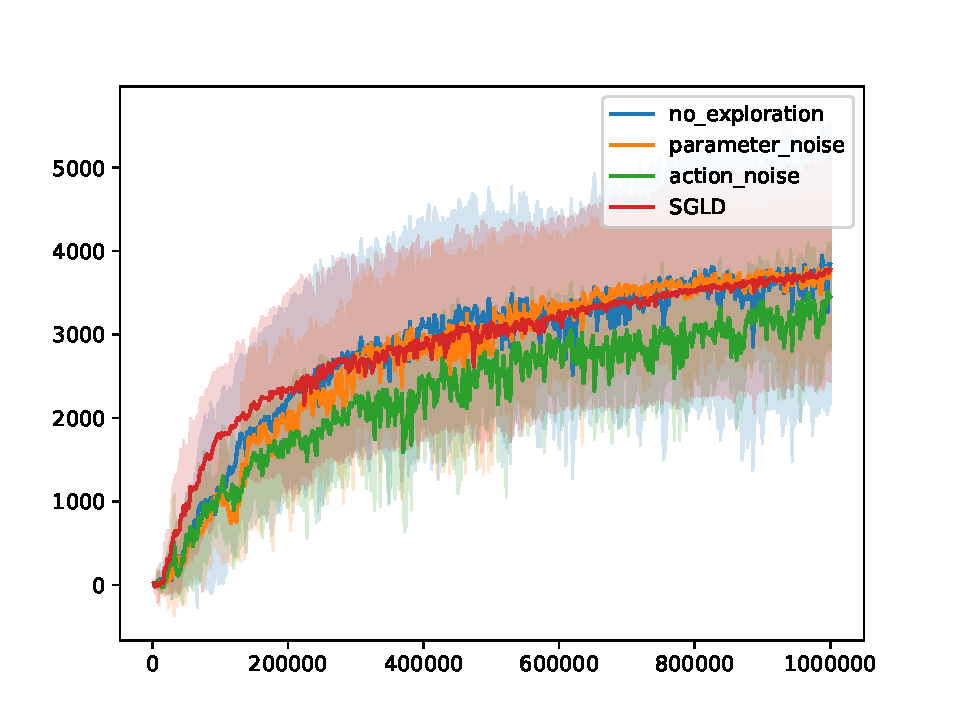
\includegraphics[width=85pt]{figs/HC0.pdf}}
      \subfigure[$\alpha = 0.1$]{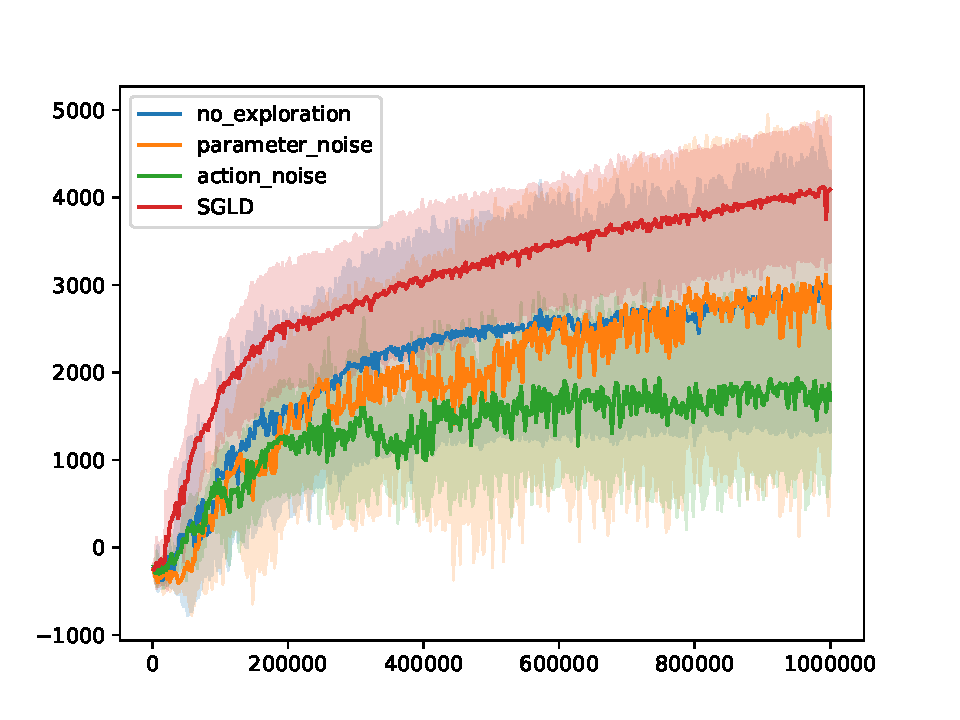
\includegraphics[width=85pt]{figs/HC.pdf}}
      \subfigure[$\alpha = 0.2$]{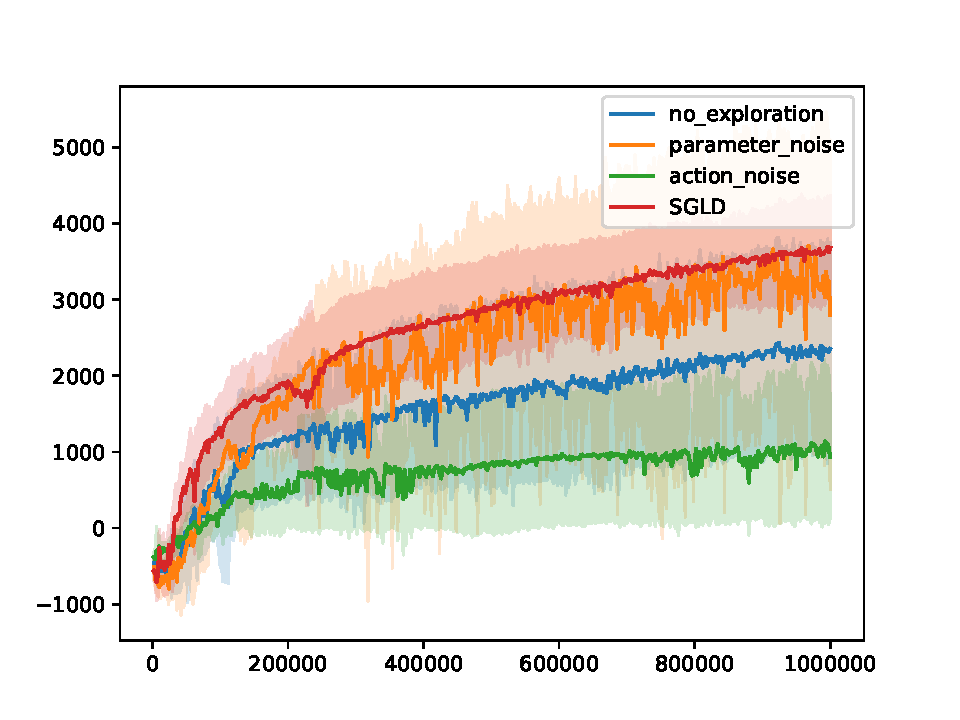
\includegraphics[width=85pt]{figs/HC0_2.pdf}}
      \subfigure[$\alpha = 0.5$]{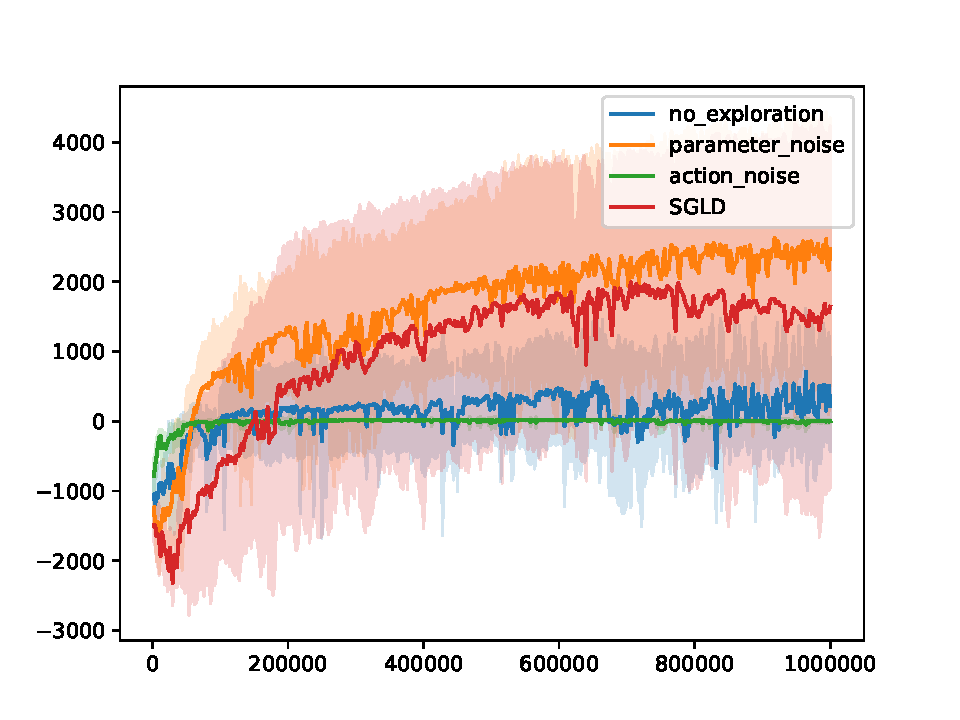
\includegraphics[width=85pt]{figs/HC0_5.pdf}}
      \subfigure[$\alpha = 1$]{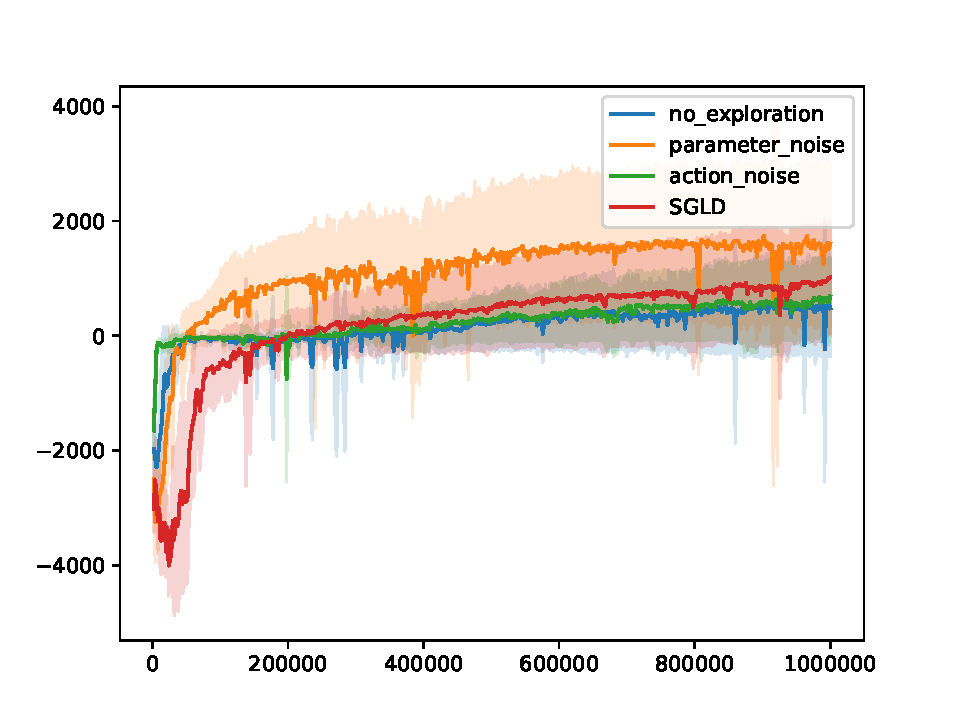
\includegraphics[width=85pt]{figs/HC1.pdf}}

      \subfigure[$d = 1$]{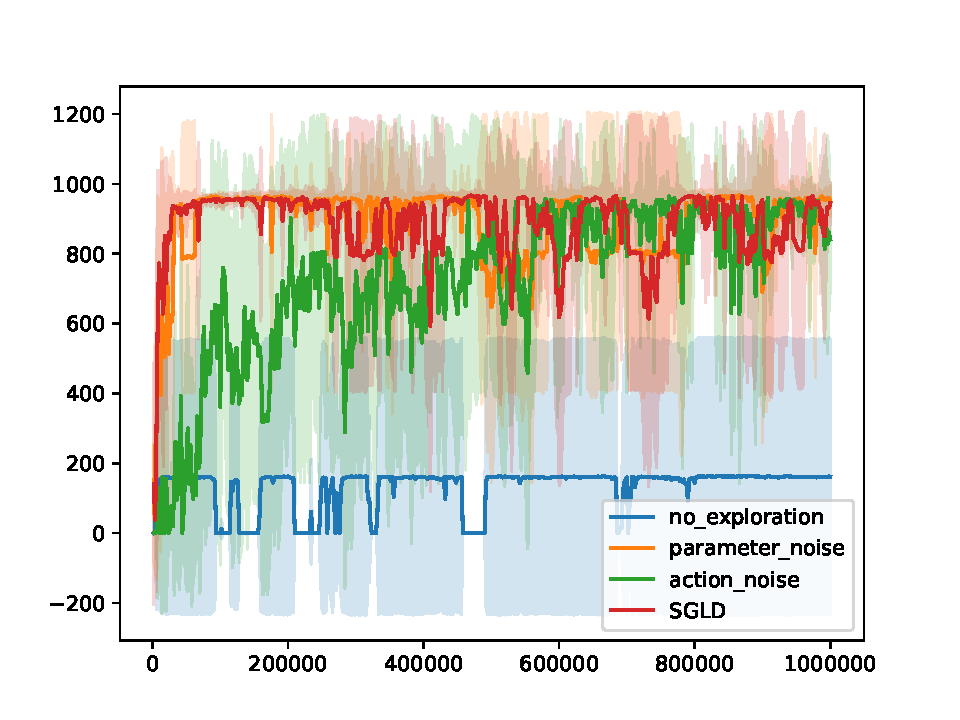
\includegraphics[width=85pt]{figs/SHC1.pdf}}
      \subfigure[$d = 2.5$]{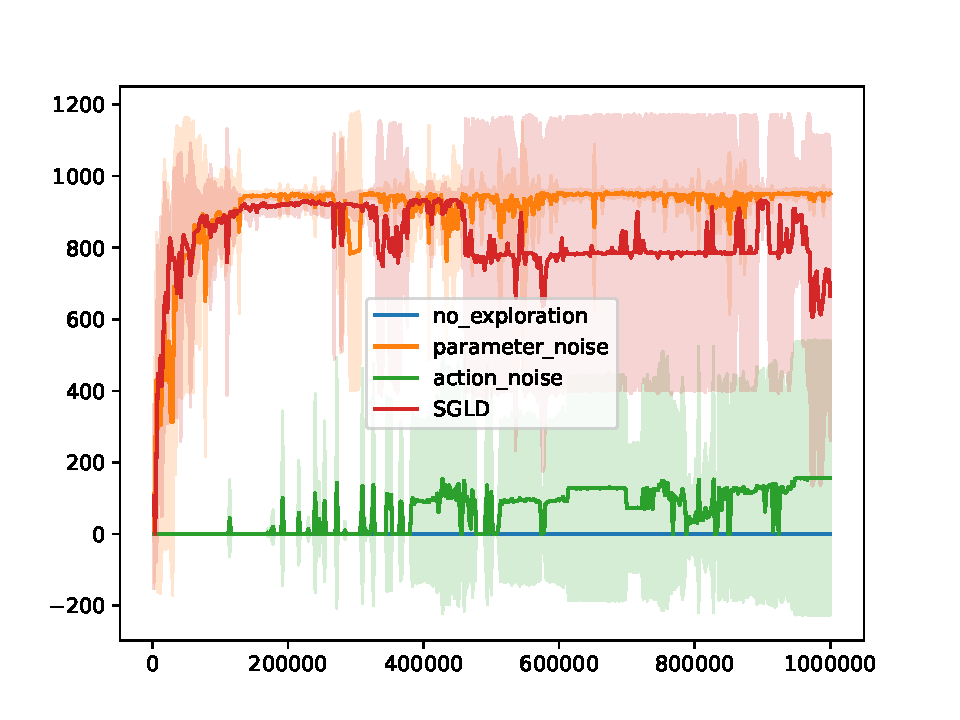
\includegraphics[width=85pt]{figs/SHC2_5.pdf}}
      \subfigure[$d = 5$]{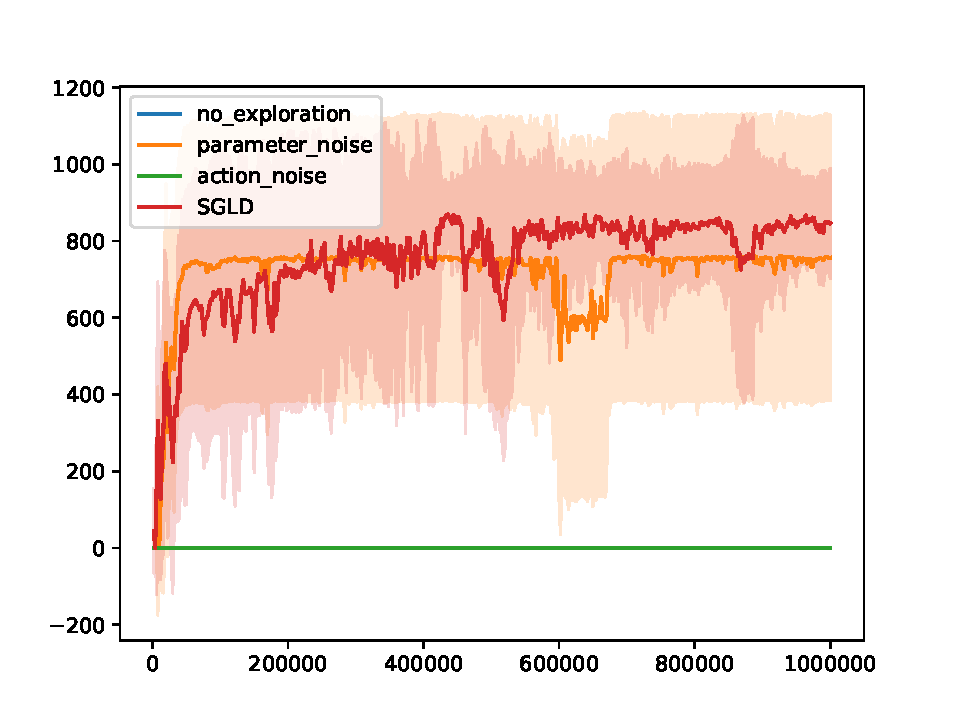
\includegraphics[width=85pt]{figs/SHC.pdf}}
      \subfigure[$d = 10$]{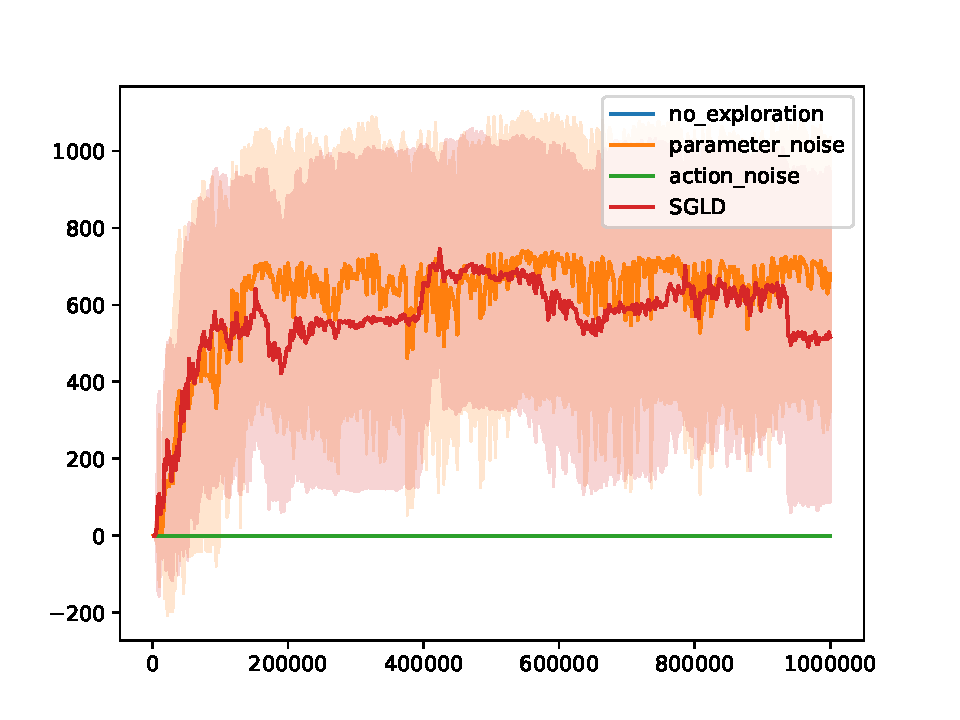
\includegraphics[width=85pt]{figs/SHC10.pdf}}
      \subfigure[$d = 20$]{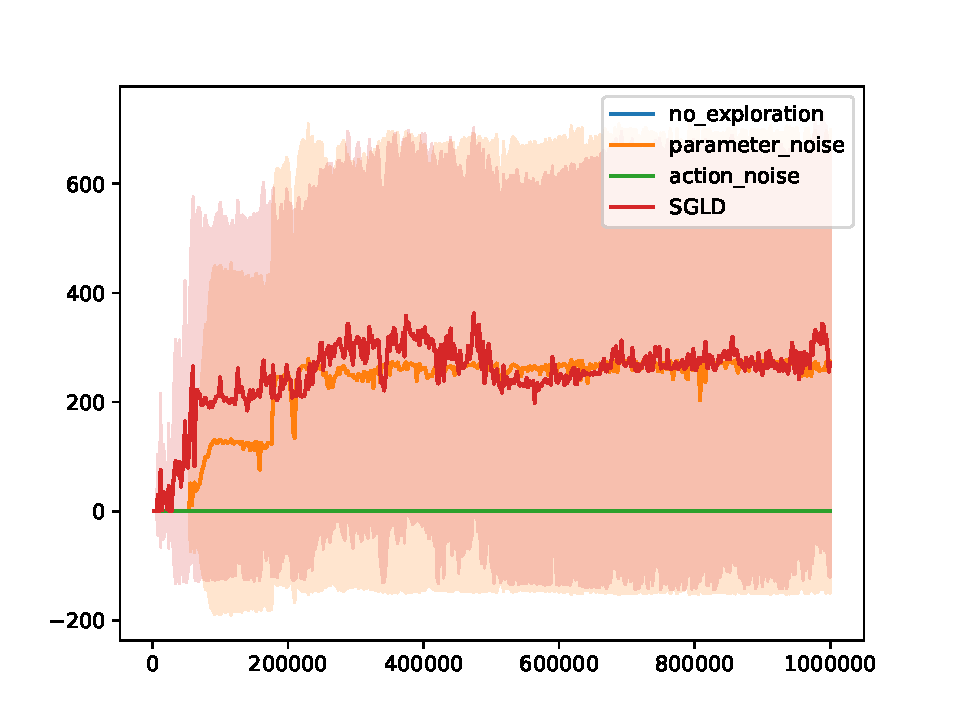
\includegraphics[width=85pt]{figs/SHC20.pdf}}
   \label{fig:allfigure}   
   \caption{Sparse HalfCheetah, $d$ is the distance between starting point and the finish line.}
\end{figure*}